% Part: sets-functions-relations
% Chapter: relations
% Section: graphs

\documentclass[../../../include/open-logic-section]{subfiles}

\begin{document}

\olfileid{sfr}{rel}{grp}
\olsection{图}

\emph{图}是一种由点——称为“节点”或“顶点”——通过边连接而成的图示。
图是离散数学与计算机科学中无处不在的工具。
它们在表示和可视化各种关系与结构方面极其有用，从各类网络等具体事物，到决策的可能结果等抽象结构。
文献中有许多不同种类的图，例如，它们的区别可能在于：边是否有向、是否有标签、是否允许从一个节点到其自身的边、相同节点之间是否允许多条边，等等。
\emph{有向图}与关系有着特殊的联系。

\begin{defn}[有向图]
\emph{有向图} $G = \tuple{V, E}$ 是由\emph{顶点}集合~$V$ 与\emph{边}集合~$E \subseteq V^2$ 构成的一个有序对。
\end{defn}

\begin{explain}
根据我们的定义，一个图就是一个集合连同该集合上的一个关系。
当然，在谈论图时，自然会期望它们能被图形化地表示：
当且仅当 $\tuple{v_1, v_2} \in E$ 时，我们就用箭头连接两个顶点~$v_1$ 和 $v_2$，以此来绘制图。
关系本身与图唯一的区别在于，图指定了顶点的集合，也就是说，图中可能包含\emph{孤立顶点}。
然而，重要的一点是，集合~$X$ 上的每个关系~$R$ 都可以看作有向图 $\tuple{X, R}$，
反之，有向图~$\tuple{V, E}$ 也可以看作是关系 $E \subseteq V^2$，只是显式地指定了集合 $V$。
\end{explain}

\begin{ex}
图 $\tuple{V, E}$，其中 $V = \{1, 2, 3, 4\}$，$E = \{\tuple{1,1}, \allowbreak \tuple{1, 2}, \allowbreak \tuple{1, 3}, \allowbreak \tuple{2, 3}\}$，图示如下：
\begin{align*}
& 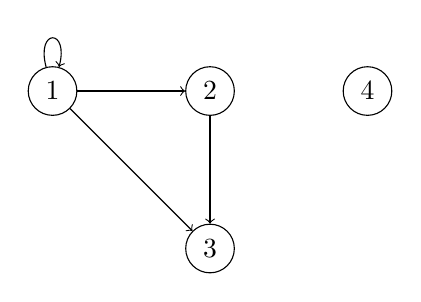
\begin{tikzpicture}[->,node distance=2cm]
  \node[draw,circle] (A) {$1$};
  \node[draw,circle] (B) [right of=A] {$2$};
  \node[draw,circle] (C) [below of=B] {$3$};
  \node[draw,circle] (D) [right of=B] {$4$};
  \draw (A) to [loop above]  (A);
  \draw (A) to  (B);
  \draw (A) to  (C);
  \draw (B) to  (C);
  \end{tikzpicture}
\intertext{这与图 $\tuple{V', E}$ 不同，其中 $V' = \{1, 2, 3\}$，图示如下：}
& 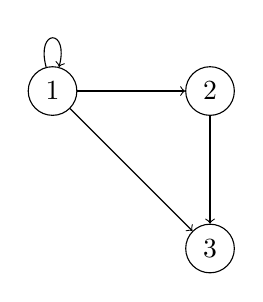
\begin{tikzpicture}[->,node distance=2cm]
  \node[draw,circle] (A) {$1$};
  \node[draw,circle] (B) [right of=A] {$2$};
  \node[draw,circle] (C) [below of=B] {$3$};
  \draw (A) to [loop above]  (A);
  \draw (A) to  (B);
  \draw (A) to  (C);
  \draw (B) to  (C);
  \end{tikzpicture}
\end{align*}
\end{ex}

\begin{prob}
  将集合 $\{1,
  2, 3, 4\}$ 上的小于等于关系~$\le$ 视为一个图，并画出对应的图示。
\end{prob}

\end{document}